	
\subsection*{Information and the Checkerboard}
	We begin by developing two fundamental measures of information theory, the entropy of one random variable and the mutual information of two. Let $X$ be a spatial variable, such as a set of coordinates in space or a neighborhood name. Let $Y$ be a compositional variable that we aim to study, defined on an alphabet $\mathcal{Y}$. In the simple case in which $\mathcal{Y}  = \{\text{Black, White}\}$, Figure \ref{fig:toy} illustrates a range of possible joint distributions $p(X,Y)$. Comparing the completely undiverse city (a) and the spatially uniformly diverse (b) motivates the first fundamental information measure, the entropy:
	\begin{equation}
		H(Y) \triangleq -\E_Y[\log p(Y)] = - \sum_{y \in \mathcal{Y}} p(y) \log p(y)\;.
	\end{equation}
	The entropy measures how evenly the global marginal distribution $p(Y)$ is distributed over the alphabet $\mathcal{Y}$. Epistemically, $H(Y)$ measures the difficulty in guessing the random variable $Y$, given no further information. $H(Y) = 0$ when $Y$ always takes a single value, such as in city (a) -- perfect guessing is possible. On the other hand, $H(Y)$ achieves its maximum of $H(Y) = \log \abs{\mathcal{Y}}$ when $Y$ is uniformly distributed on $\mathcal{Y}$, as in city (b). The entropy $H(Y)$ is this sufficient to distinguish the presence of global diversity from its absence. On the other hand, the entropy $H$ is unable to distinguish between the spatial uniformity of (b) and the spatially variability of (c). To distinguish these two cities we may use the mutual information, which is defined in terms of the Kullback-Leibler divergence $D$:
	\begin{align}
		D[p(Z)\|q(Z)] &\triangleq \sum_z p(z) \log \frac{p(z)}{q(z)} \\
		I(X,Y) &\triangleq D[p(X,Y) \| p(X)p(Y)] = \E_X[D[p(Y|X)\|p(Y)]]
	\end{align}
	Though not a true metric, the divergence $D$ is interpretable a measure of distance in the space of probability distributions, and so $I(X,Y)$ may be interpreted as the distance between the true joint distribution $p(X,Y)$ and the product of marginals $p(X)p(Y)$. Since the latter expresses statistical independence between $X$ and $Y$, $I(X,Y)$ measures the extent to which $X$ and $Y$ are dependent. Epistemically, $I(X,Y)$ measures the extent to which knowledge of $X$increases possible accuracy in guessing $Y$. In city (b), $X$ and $Y$ are independent: knowing $X$ (where an individual lives) conveys no information about that $Y$ (that individual's race).  In city (c), on the other hand $X$ and $Y$ are completely dependent: if you know where someone lives, you know their race with 100\% confidence, and $I(X,Y)$ achieves its maximum. 

	City (d) shares with city (c) the fact that race is completely determined by residence. However, city (d) embodies the ``checkerboard problem'': measures that use only the joint distribution $p(X,Y)$ without additionally considering the spatial information contained within $X$ will evaluate city (d) to be the same as city (c), despite their considerably different patterns of racial separation and potentially very different implications for planning and policy. A recent working paper \cite{Roberto2015} provides one highly operational approach to this problem, using road network topology and a weighting function that decays with distance to define a localized measure based on the Kullback-Leibler divergence. Here we pursue an alternative strategy, showing that a localization of the mutual information both measures spatial variation in race and corresponds to the estimation of a fundamental statistical property of the distribution $p(X,Y)$. 

	\begin{figure}
		\centering
		  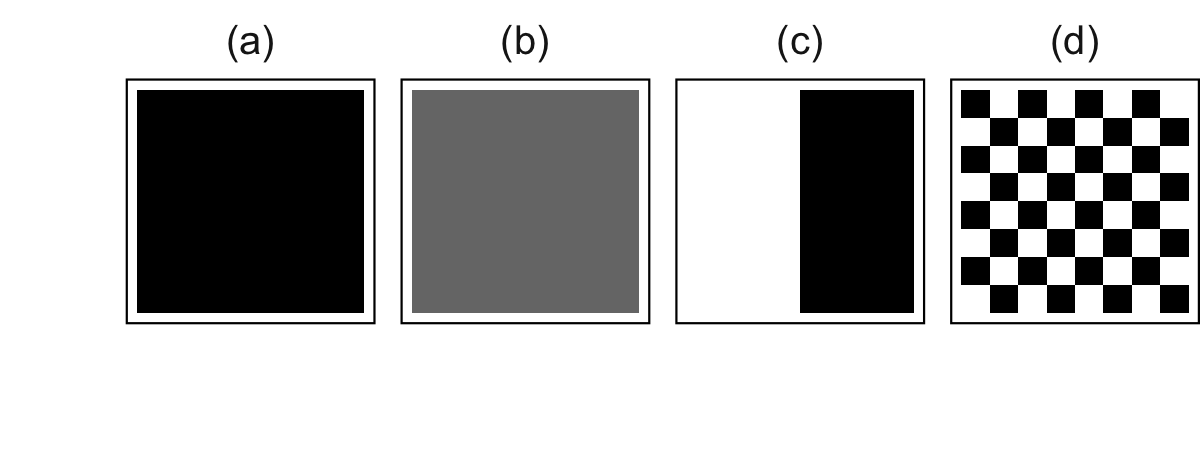
\includegraphics[width=.7\linewidth]{figs/checkerboard.png}
		\centering
		  \begin{tabular}{c | c c c}
			  City & $H(Y)$ & $I(X,Y)$ & $J(X,Y)$ \\
			  \hline			
			  (a) & 0.0 & 0.0 & 0.0\\
			  (b) & 0.7 & 0.0 & 0.0\\
			  (c) & 0.7 & 0.7 & 0.6\\
			  (d) & 0.7 & 0.7 & 2.7\\
			  \hline  
			\end{tabular}
		\caption{Information theory and the checkboard problem: model cities with various kinds of spatial diversity can be distinguished through progressively more subtle spatial information measures.}
		\label{fig:toy}
		\end{figure}

\subsection*{Measuring Socio-Spatial Complexity}

	We will now derive a measure that solves the ``checkerboard problem'' by distinguishing the toy cities (c) and (d). To motivate our methods, we  consider an idealized scenario in which we have a differentiable field $p(y|x)$ of observed probability distributions for each $x \in M \subset \R^n$, where the metric space $M$ is interpretable as the ``map'' on which we work. 

	Fix a point $x_0 \in M$ and a radius $r > 0$. Let $B_r(x_0)$ denote the ball of radius $r$ about $x_0$. Then, define the \emph{local mutual information in radius $r$} as the mutual information between $X$ and $Y$, restricted to the small ball $B_r(x_0)$ about $x_0$:
	\begin{equation}
		I_r(x_0) \triangleq \E_X[D[p(\cdot|X)\| p(\cdot|X \in B_r(x_0))]|X \in B_r(x_0)] \label{eq:local}
	\end{equation}
	Intuitively, $I_r(x_0)$ measures how much knowing the ``location'' $x$ adds to our information about the category $Y$, or, equivalently, how much the probability field $p(y|x)$ varies with $x$ in a small neighborhood of $x_0$. It is therefore a natural measure of local complexity, aligned in approach with the global mutual information but designed to detect local variation. As expected, $I_r(x_0) = 0$ if and only if $p(y|x)$ is constant for each $y$ in the ball $B_r(x_0)$; that is, if within $B_r(x_0)$ the field $p(y|x)$ resembles toy city (b) in Figure \ref{fig:toy}. In the definition \eqref{eq:local}, $r$ may be thought of as the spatial resolution at which we conduct analysis, and $I_r(x_0)$ is highly dependent on $r$. However, it is possible to show that $I_r(x_0)$ is related to a fundamental statistical property of the probability field $p(y|x)$ that is resolution-independent. Under the stated conditions, the following approximation holds: 

	\begin{equation}
		\frac{I_r(x)}{r^2} \cong \frac{1}{4} \text{trace } J_Y(x)\;, \label{eq:approx}
	\end{equation}
	where $J_Y(x)$ is the Fisher information matrix in $Y$ about $x$, defined as 
	\begin{equation}
		J_Y(x) \triangleq \E_Y\left[ (\nabla_x \log p(Y|x))(\nabla_x \log p(Y|x))^T \right]\;.
	\end{equation}
	A formal statement and proof of \eqref{eq:approx} are provided in Appendix 2. The Fisher information $J_Y$ is a fundamental quantity in statistics and information theory. From a geometric perspective, $J_Y$ provides the natural intrinsic metric in the geometric space of probability distributions parameterized by the spatial variable $x$. Equation \eqref{eq:approx} therefore expresses a relationship between the local mutual information $I_r(x)$ and the information geometry of the underlying probability field. Corresponding to the fact that $I_r(x_0)$ vanishes if and only if $p(y|x)$ is constant in $B_r(x_0)$, $J_Y(x_0) = 0$ if and only if $\nabla_x p(y|x_0) = 0$ for all $y$. This implies that $x_0$ is a stationary point, about which the probability field $p(y|x_0)$ exhibits only small (2nd order or smaller) changes with respect to changes in $x$. 

	Since the Fisher information is a strictly local measure of statistical variability around $x$, we can aggregate the Fisher information to derive a measure of average local variability. The \emph{mean local information} is 
	\begin{equation}
	J(X,Y) \triangleq \E_X[\text{trace }J_Y(X)] \label{eq:def_J}
	\end{equation} 
	As demonstrated in Figure \ref{fig:toy}, $J(X,Y)$ distinguishes cities (c) and (d), thereby addressing the ``checkerboard problem'' head on. We propose the aggregate quantity $J(X,Y)$ as a third  measure--alongside the entropy $H(Y)$ and mutual information $I(X,Y)$-- as a tool for the information-theoretic structure of spatial compositional complexity. 

	We note that, since 
	\begin{align}
		\text{trace } J_Y(x) &= \E_Y\left[ \norm{\nabla_x \log p(Y|x)}^2 \right]\;
	\end{align}
	may be viewed as the average norm of the gradient of $\log p(Y|x)$, the quantity  
	\begin{align}
		J(X,Y) &= \E_X[\text{trace } J_Y(X)] \\
		&= \E_{X,Y}\left[\norm{\nabla_x \log p(Y|X)}^2\right]
	\end{align}
	may be viewed as a cousin to total variation measures often encountered in mathematical analysis. 

	While we have developed these methods in the context of a differential field of observed distributions $p(y|x)$, their application to a discrete data set is conceptually simple. For a given set of tracts, overlay an evenly spaced grid of radius $r$, and measure the mutual information $I_r(x)$ in each grid cell. Then, when data and grid resolutions are sufficiently high, $4I_r(x) / r^2$ approximates the quantity $\text{trace }J_Y(x)$, which can then be aggregated across the data set. We provide a more formal statement of this computation in the appendix. 

\subsection*{Information Measures and Segregation Studies}

	Considerable attention has been paid to relating segregation indices to intuitive concepts of diversity and segregation. In this section, we relate the information measures $H(Y)$, $I(X,Y)$, and $J(X,Y)$ to three standard dimensions of diversity and segregation in sociology. In brief,
	\begin{itemize}
		\item The entropy $H(Y)$ measures global diversity. 
		\item The mutual information $I(X,Y)$ measures \emph{evenness}. 
		\item The local information $J(X,Y)$ measures \emph{spatial exposure}. 
	\end{itemize}
	We will define the latter two terms and argue for these claims below. In doing so, we make a case for these measures as practical tools in the quantitative study of urban diversity. 

	One way to quantify diversity is to consider how closely the distribution of races resembles the uniform distribution. A ``maximally diverse'' city might be 20\% each Asian, Black, Hispanic, Other, and White. The entropy measures distance from the uniform distribution, as can be formalized through the identity: 
	\begin{equation}
		H(Y) = \log \abs{\mathcal{Y}} - D[p(Y)\|u(Y)]
	\end{equation}
	where $u$ is the uniform distribution on $\mathcal{Y}$. The entropy is thus largest when the distribution $p(Y)$ is nearly uniform, and smallest when $p(Y)$ is ``farthest'' from the uniform distribution. Through properties of $D$, it is possible to show that these cases occur when $p(Y)$ is itself uniform and when $Y$ is a constant, respectively. Since entropy measures nearness to uniformity, it is an intuitive characterization of the idea of diversity. 

	We now turn to the relationship between the mutual information $I(X,Y)$ and sociospatial evenness. The authors of \cite{Reardon2002} define \emph{spatial evenness} as ``the extent to which groups are similarly distributed in residential space'' (page 126), and argue that this concept encapsulates those of clustering, concentration, and centralization used in \cite{Massey1988}. To see that $I(X,Y)$ measures (un)evenness, consider the model cities (b) and (c) in Figure \ref{fig:toy}. In city (b), knowing where a person lives carries no information about their race, in the sense that, if you are attempting to guess someone's race, learning their residence will be of no help to you. In contrast, in city (c), location determines race: if you learn a person's residence, you can guess their race with 100\% accuracy. This difference is cast in information terms, but it is precisely the difference between evenness and unevenness. In (c), location epistemically determines race precisely because races are unevenly distributed across locations. 

	Finally, we consider the local information $J(X,Y)$ and its connection to spatial exposure. The authors of \cite{Reardon2002} define \emph{spatial exposure} as ``the extent that members of one group encounter members of another group...in their local spatial environments'' (page 126). Our contention is that $J(X,Y)$ measures exposure conditional on a fixed level of evenness (as measured by $I(X,Y)$). To see this, consider cities (c) and (d) in Figure \ref{fig:toy}. These cities are equally diverse as measured by $H(Y)$ and equally uneven as measured by $I(X,Y)$. The difference between them is that (c) consists of two large, racially-distinct neighborhoods, of which only residents near the center are exposed to residents of the other. On the other hand, in (d), all residents are just one ``block'' away from residents who do not share their race. $J(X,Y)$ detects this difference because the localized mutual information $I_r$ in terms of which $J(X,Y)$ is defined precisely as the unevenness in a small area. We should emphasize, however, that $J(X,Y)$ should always be considered in the context of $I(X,Y)$. City (d) clearly has more exposure than (c), but less than the perfectly even (b). The difference is that (b) has no neighborhood structure at all. 

	This point highlights that, though the concepts of diversity, evenness, and exposure are conceptually distinct, they are not fully independent. There exists a hierarchical relationship among them. Complete lack of diversity ($H(Y) = 0$) implies perfect evenness ($I(X,Y) = 0$), as in city (a). In turn, perfect evenness implies maximal exposure, but also a lack of neighborhood structure $J(X,Y)$, as in city (b). While this point may appear theoretical, it is necessary to keep in mind in the context of practical data analysis. Interpreting whether or not $I(X,Y)$ is ``high'' in a given city requires contextualizing its value against $H(Y)$. Similarly, evaluating a value of $J(X,Y)$ requires keeping $I(X,Y)$ in mind. 

\subsection*{Properties of Information Diversity Measures}
	There has been much work showing the desirable properties of various segregation indices. To give a brief sampling, many scholars agree that such indices should be invariant to changes in overall population size; they should decrease when populations ``even themselves out,'' and they should behave predictably under aggregation. How do the measures $I(X,Y)$ and $J(X,Y)$ compare? The author of \cite{Roberto2015a} shows that the mutual information $I(X,Y)$ (which she calls the ``Divergence Index'') satisfies the core desiderata of segregation indices, generally as well or better than existing alternatives. We highlight one property of $I(X,Y)$ for special note, as it will be central to our development of natural neighborhood identification. The principle of ``additive decomposability'' \cite{Reardon2002} stipulates that, when the data is grouped along either racial or spatial axes, a good segregation index should split into ``within group'' and ``between group'' components. In the context of the mutual information $I(X,Y)$, additive decomposability is simply the familiar chain rule of mutual information. For concreteness, let $C$ be a random variable giving the cluster label of location $X$; importantly, $C$ is completely determined by $X$. Then, the chain rule expresses additive decomposability as 
	\begin{equation}
		I(X,Y) = I(C,Y) + I(X,Y|C)\;; \label{eq:information_decomp}
	\end{equation}
	This information identity has a simple epistemic interpretation: he information I have about someone's race $Y$ given that I know their residence $X$ is equal to the information I have if I first learn their broad neighborhood $C$, plus the amount of additional information I gain if I subsequently learn the exact residence $X$ as well. Mathematically, this expression decomposes $I(X,Y)$ into two useful components. The first term is interpretable as the between-group information, while the second is interpretable as the within-group information. It is therefore comparable to the familiar between-group/within-group ``sum of squares'' decompositions that frequently appear in classical statistical analysis. A similar version of the chain rule expresses additive decomposability for aggregation of racial groups rather than spatial locations. In the next subsection, we use \eqref{eq:information_decomp} to define a clustering procedure to identify natural neighborhoods in cities. 

	We now turn to the properties of $J(X,Y)$. Our core argument is that $J(X,Y)$ possesses a variety of intuitive properties, and that those it does not either underscore the importance of reading it in conjunction with $I(X,Y)$ or need not apply to spatialized measures.  See \cite{Reardon2002,Reardon2004} for detailed discussion of these criteria. 
	\begin{description}
		\item[Organizational Equivalence:] Both the theoretical definition \eqref{eq:def_J} and the procedure to compute it from discrete data remain unchanged when a tract is subdivided into smaller tracts, each of which with identical demographic structure. 
		\item[Size and Density Invariance:] Since $J(X,Y)$ is completely determined by the probability measure $p(X,Y)$, it is invariant under global changes in population density. 
		\item[Additive Group Decomposability:] When demographic groups are aggregated into super-groups, the chain rule of mutual information applied to the demographic variable $Y$ provides an an additive decomposition of the form $J(X,Y) = J(X,G) + J(X,Y|G)$ for the mean local information. This can be interpreted as a sum of between-groups and within-gropus terms as required. 
		\item[Scale Interpretability:] We have $J(X,Y) = 0$ if and only if $p(Y|X)$ is constant on each connected component of the metric space $M$. When only one connected component exists, this implies that every locale has the same demographic structure as the global environment. When multiple connected components exist (e.g. the city is divided by a river), demographics must be constant in space on each side of the division. $J(X,Y)$ does not achieve its maximum value when all locales are monoracial, but this point only emphasizes that $J(X,Y)$ and $I(X,Y)$ should be read jointly. When all locales are monoracial, $I(X,Y)$ achieves its maximum value and $J(X,Y) = 0$. 
		\item[Boundary Independence:] $J(X,Y)$ is defined in terms of a continuous underlying probability distribution $p(X,Y)$, rather than arbitrarily-defined tracts. In computational practice, $J(X,Y)$ is indeed sensitive to the boundaries supplied with the data; however, \eqref{eq:approx} guarantees that this sensitivity vanishes as the resolution grows sufficiently small. No alternative measure can overcome limited data resolution, and, to our knowledge, no other measure comes with the same assurance of limiting resolution independence. 
		\item[Transfers and Exchanges:] The core idea of the principles of transfers and exchanges is that population permutations that tend to ``smooth out'' differences should reduce segregation measures. No strict such condition holds for $J(X,Y)$; however, this is comparatively not a large limitation, as most of the measures considered in \cite{Reardon2004} also fail to meet rigorous transfer and exchange principles. $J(X,Y)$ does satisfy the following useful and interpretable criterion: when a transfer makes all affected areas more closely resemble their immediate neighbors, $J(X,Y)$ decreases. Notably, these transfers can tend to either increase or reduce spatial evenness, and $I(X,Y)$ may increase or decrease accordingly. 
		\item[Additive Spatial Decomposability:] This criterion states that ``If X spatial subareas are aggregated into Y larger spatial areas, then a segregation measure should be decomposable into a sum of within- and between-area components'' \cite{Reardon2004}, page 136. However, considering that we have imposed additional spatial structure on our model, this criterion does not appear to be motivated. Consider, for example, Figure \ref{fig:decomposability}. Aggregating the two central regions transforms (e) into (f), erasing all spatial variability. Any measure should therefore have a between-groups component equal to 0. On the other hand, the within-groups component can only consider the middle white/black boundary between the central two regions. The sum of the between-groups and within-groups components must therefore consist only in information included in the middle boundary. However, the spatial variability in city (e) is not exhausted by this middle boundary; there are a total of six other frontiers of racial difference that should be considered in any spatial segregation measure. We therefore content that additive decomposability is a desideratum of nonspatial measures (it is satisfied by $I(X,Y)$), but not of explicitly spatial ones. 
	\end{description}
	
	\begin{figure}
		\centering
		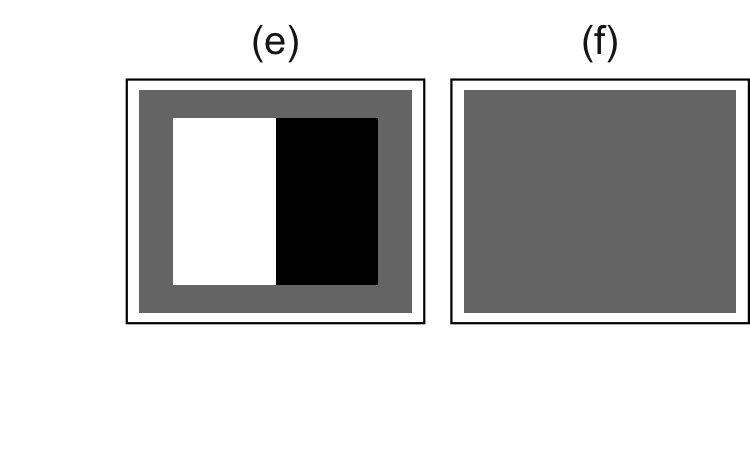
\includegraphics[width=.5\textwidth]{figs/decomposability.png}
		\caption{A problem with additive spatial decomposability: aggregating the inner two regions transforms (e) into (f), smoothing out all spatial variability. A ``between groups'' term must therefore vanish, while a ``within-groups'' term considers only the inner boundary; not the outer ones.}
		\label{fig:decomposability}
	\end{figure}
	
	In summary, $J(X,Y)$ possesses a variety of useful, intuitive properties. The ones it fails to possess reflect the fact that these desiderata are typically formulated to apply to a single measure. While we have not exhausted the full complement of desiderata for segregation measures. However, many of the remaining ones -- such as composition invariance -- are either difficult to define mathematically or controversial within the sociological community, and we will not them consider further. 

	We close with a discussion of some of the theoretical and operational virtues of $I(X,Y)$ and $J(X,Y)$ not considered above. 
	\begin{description}
		\item[Interpretability:] In contrast to many previous works, we make no attempt to encapsulate every aspect of diversity in a single measure. The result of maintaining distinct measures is that each of our two separate measures are highly interpretable. The mutual information $I(X,Y)$has a standard interpretation in information theory: it is the epistemic value of knowing where an individual lives for the purposes of predicting their race, as measured using the logarithmic loss function; see \cite{Cover1991} for a detailed discussion of information measures and prediction. The local information $J(X,Y)$ is then interpretable as the epistemic value of knowing where an individual lives when restricting one's attention to a small area. The direct operational meaning of these metrics is the source of their desirable mathematical properties, and reflects the virtue of starting from a unified mathematical framework.  
		\item[Kernel Independence:] Many existing spatial information measures depend on a choice of spatial kernel function which serves as a functional definition of proximity. While providing flexibility, dependence on a spatial kernel function increases researcher degrees of freedom and makes it more difficult to compare studies. There is no theoretical consensus on the appropriate kernel. The mutual information $I(X,Y)$ is aspatial and requires no kernel. In practice, computing $J(X,Y)$ does require a choice of a grid radius (see Appendix for details), but does not require the specification of a functional kernel. 
		\item[Isotropy:] As a result of its kernel independence, $J(X,Y)$ is \emph{isotropic}, taking no consideration of natural boundaries or infrastructure. This property has both virtues and drawbacks. On the one hand, an isotropic measure is simple to compute, simple to interpret, and easily generalized. On the other, boundaries and infrastructure unquestionably shape interactions between people, and are clearly relevant in segregation studies. We note, however, that most urban anisotropies exist on the scale of a few hundred meters at most. Therefore, we expect that anisotropic measures will only be relevant at scales of analysis substantially smaller than the 500m used in this study. A detailed numerical comparison of isotropic and anisotropic measures would be most welcome. 
		\item[Connection to Data Analysis:] As we will see below, the mutual information $I(X,Y)$ can be used to define a practical algorithm for the identification of natural, demographically coherent neighborhoods, and the local information $J(X,Y)$ predicts its performance. These two measures are thus not only of theoretical interest, but also provide tools for the practical analysis of urban diversity. We are not aware of any other measures that share this helpful property. 
	\end{description}

	\begin{figure}
		\begin{tabular}{l | c c c}
		Criterion & $H(Y)$ & $I(X,Y)$ & $J(X,Y)$ \\
		\hline
		Scale Interpretability & \checkmark & \checkmark & \checkmark \\
		Density Invariance & & & \\
		Compositional Invariance & & & \\
		Transfers & & & \\
		Additive Organizational Decomposability & & & \\
		Additive Spatial Decomposability & & & 
		\end{tabular}
	\end{figure}


\subsection*{Identifying Natural Neighborhoods} 
	
	Equation \eqref{eq:information_decomp} motivates a simple scheme for identifying natural neighborhoods based on maximizing the between-group term $I(C,Y)$. If all I had access to were the cluster labels $C$ and not the locations $X$, then the information I had about $Y$would be $I(C,Y)$. A ``good'' clustering therefore maximizes the between-cluster information $I(Y,C)$, which entails minimizing the within-cluster information $I(X,Y|C)$. Solving this problem exactly is a challenging discrete optimization problem, and may not be computationally tractable. We can, however, construct a greedy algorithm which leads to satisfactory results. At each stage of the algorithm, we consider the problem of choosing a pair of tracts $\{i*,j*\}$ to cluster together. The reduction in information associated with aggregating the locations $I$ into a single cluster is 
	\begin{align}
		d(i,j) &\triangleq  \sum_{k \in \{i,j\}} p(X = k)D[p(Y|X = k)\| p(Y|X \in \{i,j\})] \\
		&- p(X\in \{i,j\})D[p(Y|X\in \{i,j\}) \| p(Y)] \label{eq:info_dist}
	\end{align}
	where $p(Y) = \sum_{x} p(x,Y)$ is the global marginal distribution. the first term is the information associated with the two separate tracts, while the second is the information associated with a merged tract. Equation \eqref{eq:info_dist} defines a natural information distance between locations $i$ and $j$. Like the KL divergence, this distance is strictly nonnegative; unlike the KL divergence, it is symmetric, and defines an axiomatic metric on the space of tracts. Importantly, we can therefore use the distance $d(i,j)$ as a dissimilarity measure for the purposes of clustering. Our greedy procedure is simple: at each iteration, determine
	\begin{equation}
		(i^*,j^*) = \argmin_{i \text{ neighbors } j} d(i,j),
	\end{equation}
	and then combine $i^*$ amd $j^*$ into a single tract, repeating until only one cluster remains. This procedure defines a form of agglomerative hierarchical clustering distinguished by two characteristics: its spatial constraints and its pursuit of minimal information loss at each step. As a greedy algorith, it possesses no guarantees for optimal solutions, but in practice its performance leads to intuitive, racially-coherent regions. It thereby enables a study of spatial difference using non-arbitrarily-defined regions. 






